% --------------------------------------
% Document Class
% --------------------------------------
\documentclass[a4paper,11pt]{article}
% --------------------------------------



% --------------------------------------
% Use Package
% --------------------------------------


\usepackage[francais]{babel}
%\usepackage{ucs}
\usepackage[utf8]{inputenc}
\usepackage[T1]{fontenc}

\usepackage{makeidx}
\usepackage{color}
\usepackage{graphicx}
\usepackage{float}
\usepackage[hidelinks]{hyperref} 
\usepackage{geometry}
%\usepackage{lastpage}
%\usepackage{marginnote}
\usepackage{fancyhdr}
%\usepackage{titlesec}
%\usepackage{framed}
\usepackage{amsmath}
\usepackage{empheq}
\usepackage{array}
\usepackage{multicol}
\usepackage{csquotes}
%\usepackage{adjustbox}

% insert code
\usepackage{listings}

% define our color
\usepackage{xcolor}

% code color
\definecolor{ligthyellow}{RGB}{250,247,220}
\definecolor{darkblue}{RGB}{5,10,85}
\definecolor{ligthblue}{RGB}{1,147,128}
\definecolor{darkgreen}{RGB}{8,120,51}
\definecolor{darkred}{RGB}{160,0,0}

% other color
\definecolor{ivi}{RGB}{141,107,185}


\lstset{
    language=java,
    captionpos=b,
    extendedchars=true,
    frame=lines,
    numbers=left,
    numberstyle=\tiny,
    numbersep=5pt,
    keepspaces=true,
    breaklines=true,
    showspaces=false,
    showstringspaces=false,
    breakatwhitespace=false,
    stepnumber=1,
    showtabs=false,
    tabsize=3,
    basicstyle=\small\ttfamily,
    backgroundcolor=\color{ligthyellow},
    keywordstyle=\color{ligthblue},
    morekeywords={include, printf, uchar},
    identifierstyle=\color{darkblue},
    commentstyle=\color{darkgreen},
    stringstyle=\color{darkred},
}


% --------------------------------------



% --------------------------------------
% Page setting
% --------------------------------------
%\pagestyle{empty}
\setlength{\headheight}{15pt}

\setcounter{secnumdepth}{3}
\setcounter{tocdepth}{2}

\makeatletter
\@addtoreset{chapter}{part}
\makeatother 

\hypersetup{         % parametrage des hyperliens
  colorlinks=true,      % colorise les liens
  breaklinks=true,      % permet les retours à la ligne pour les liens trop longs
  urlcolor= blue,       % couleur des hyperliens
  linkcolor= black,     % couleur des liens internes aux documents (index, figures, tableaux, equations,...)
  citecolor= green      % couleur des liens vers les references bibliographiques
}

% --------------------------------------

% --------------------------------------
% Information
% --------------------------------------
\title{Compte-rendu TP11 TI : Formation des images couleur et dématriçage}
\author{Elliot VANEGUE et Gaëtan DEFLANDRE}
% --------------------------------------

\definecolor{myColor}{rgb}{0.5, 0.1, 0.75}

% --------------------------------------
% Begin content
% --------------------------------------
\begin{document}

% Set language to english
  \selectlanguage{francais}

  % Start the page counting
  \pagenumbering{arabic}

  \maketitle
  
  \mbox{}
  \newpage
  \clearpage
  
  \section{Introduction}
  Avant de pouvoir traiter une image, il faut pouvoir l'acquérir au moyen d'un capteur présent dans les
  caméras ou appareils photo par exemple. Dans nos appareils grand public, un capteur est composé d'une mosaîque
  de pixels. Les pixels ne peuvent représenter qu'un seul dégradé de couleur. C'est pourquoi il existe différents
  CFA\footnote{Color Filter Array} qui permettent d'obtenir une image couleur. Durant ce TP, nous allons voir
  comment est utilisé le CFA de Bayer.
  
  \section{Interprétation et simulation d'une image CFA}
  Etant donné que nous travaillons sur une image acquise avec un CFA de Bayer, nous pouvons déterminer quelle est
  la disposition des pixels de l'image. Lorsque nous regardons le coin haut gauche, qui représente un ciel bleu, nous
  constatons que le troisième pixel est plus clair que les deux premiers dans l'image CFA. Or le troisième pixel 
  a une valeur dans la composante bleu qui est plus importante que les deux premiers pixels. Donc la première configuration
  de Bayer utilisée sur notre image est la suivante : \\
  
  \begin{figure}[H]
  \center
   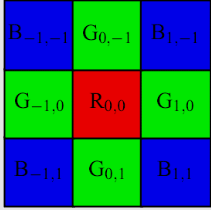
\includegraphics[width=3cm]{bayerGRG.png}
  \end{figure}

  Nous allons maintenant simuler la génération d'une image CFA à partir de l'image couleur. Pour
  cela nous appelons la méthode \enquote{cfa} qui nous est fournie et nous stockons le résultat
  dans un ImageProcessor que nous affichons. Nous obtenons ainsi une image CFA dont la configuration
  est la suivante :
  
  \begin{figure}[H]
  \center
   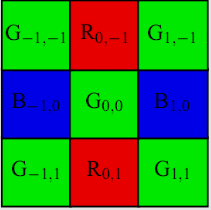
\includegraphics[width=3cm]{bayerBGB.png}
  \end{figure}
  
  Nous obtenons donc une image en dégradé de gris, car une image CFA ne comporte qu'un seul canal par pixel,
  c'est après un dématriçage que l'image possèdera trois canaux représentant chaque composante couleur.
  
  \section{Dématriçage par interpolation bilinéaire}
  
  Dans notre cas, nous traitons des images CFA dont la disposition est G-R-G. Il est donc possible de 
  retrouver les pixels de chaque plan $\varphi^k$. Par exemple, on obtient pour le début du plan rouge, 
  les pixels sur la dispositions suivante:
  
  \begin{figure}[H]
   \center
   \includegraphics[width=3cm]{phi_r_cfa_export.png}
   \caption{Disposition des pixels rouges}
  \end{figure}
  
  Nous avons dans notre cours les quatre formules de dématriçage suivantes :\\
  
  Configuration {GRG} (id. en {GBG}) :\\
  \begin{align}
  B &= \frac{1}{4} * (B_{-1,-1}+B_{1,-1}+B_{-1,1}+B_{1,1})\\
  G &= \frac{1}{4} * (G_{0,-1}+G_{-1,0}+G_{1,0}+G_{0,1})
  \end{align}
  
  Configuration {RGR} (id. en {BGB}) :\\
  \begin{align}
  R &= \frac{1}{2} * (R_{-1,0}+R_{1,0})\\
  B &= \frac{1}{2} * (B_{0,-1}+B_{0,1})
  \end{align}
  
  Nous pouvons alors déterminer les masques de convolution à appliquer sur le plan $\varphi^G$,
  pour retrouver la composante G, $\frac{1}{4}$
  $\begin{pmatrix}
   0 & 1 & 0\\
   1 & 4 & 1\\
   0 & 1 & 0
  \end{pmatrix}$
  puisque l'on peut voir dans l'équation de G qu'il a besoin de ses voisins du dessus, du dessous,
  de gauche et de droite afin de calculer le pixel courant. Pour les composantes suivantes, le calcul
  est un peu plus complexe, car leurs équations varient en fonction de la configuration du CFA. Le masque
  correspondant aux deux autres composantes est $\frac{1}{4}$
  $\begin{pmatrix}
   1 & 2 & 1\\
   2 & 4 & 2\\
   1 & 2 & 1
  \end{pmatrix}$. Dans cette matrice, les valeurs en (1,0), (0,1), (-1,0) et (0,-1) sont à 2, car 
  les équations 3 et 4 ont un coefficient non pas de $\frac{1}{4}$ mais de $\frac{1}{2}$, il faut
  donc leur donner un poids deux fois plus important que le reste des voisins. Le reste des voisins n'a 
  qu'un poids de 1 dans le masque grâce à l'équation 1.\\
  
  Nous allons maintenant effectuer un dématriçage bilinéaire sur l'image CFA que nous avons calculée
  précédement (configuration G-R-G). Pour cela nous créons trois images contenant les trois plans $\phi^k$.
  Pour calculer ces plans, nous créons une image et nous ne gardons que les pixels appartenant au plan considéré.
  Par exemple pour calculer le plan $\phi^R$ nous allons garder les pixels rouges de l'image suivante et mettre tous 
  les autres à 0.
  
  \begin{figure}[H]
  \center
   \includegraphics[width=3cm]{phi_r_cfa_export.png}
  \end{figure}

  Une fois que nous obtenons les trois images représentant chaque plan, nous pouvons leur appliquer le masque de
  convolution qui leur correspond. Pour les plans $\phi^R$ et $\phi^B$ nous utilison le masque 
  $\begin{pmatrix}
    1/4 & 1/2 & 1/4\\
    1/2 & 1 & 1/2\\
    1/4 & 1/2 & 1/4\\
   \end{pmatrix}$ et pour le plan $\phi^G$ nous utilison le masque 
   $\begin{pmatrix}
    0 & 1/4 & 0\\
    1/4 & 1 & 1/4\\
    0 & 1/4 & 0\\
   \end{pmatrix}$.
   Il reste alors à combiner les trois plans pour obtenir une image couleur.\\
   
   Nous pouvons voir sur l'image résultante que les couleurs correspondent à l'image initiale. Cependant,
   l'image comporte des couleurs aberrantes qui résultent d'un écart important entre la couleur attendue
   et la couleur calculée.

  \begin{figure}[H]
  \center
   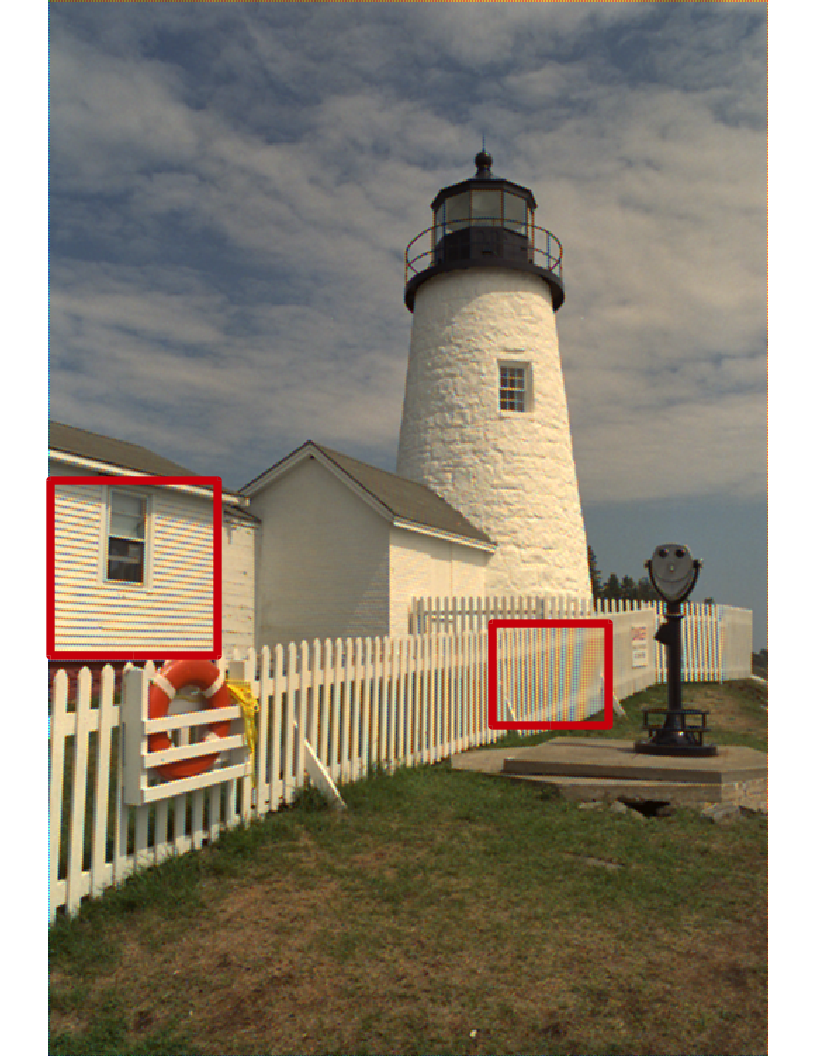
\includegraphics[width=8cm]{../result2ROI.png}
   \caption{Image après dématriçage avec la localistion des principales couleurs aberrantes}
  \end{figure}
   
  \section{Dématriçage basé sur l'estimation locale d'un gradient}
  
  \newpage
 
  \section{Annexes}
  
  \subsection{Plugin de la simulation d'un image cfa}
  
  \begin{lstlisting}[caption=Code du premier exercie]
import ij.IJ;
import ij.ImagePlus;
import ij.gui.GenericDialog;
import ij.plugin.filter.PlugInFilter;
import ij.process.ByteProcessor;
import ij.process.ImageProcessor;


public class compute_cfa implements PlugInFilter {

	// ATRIBUTES //

	public final static int	R_G_R = 0;
	public final static int	B_G_B = 1;
	public final static int	G_R_G = 2;
	public final static int	G_B_G = 3;

	/**
	 * Fenêtre contenant l'image de référence
	 */
	private ImagePlus imp;

	/**
	 * Largeur de la fenêtre
	 */
	private int width;

	/**
	 * Hauteur de la fenêtre
	 */
	private int height;

	// METHODS //

	/**
	 * Méthodes de configuration du plug-in, appelé en première. L'image sur
	 * laquelle nous travaillons est l'image de référence en couleur.
	 */
	public int setup(String arg, ImagePlus imp) {
		this.imp = imp;
		return PlugInFilter.DOES_RGB;
	}

	public void run(ImageProcessor ip) {

		// Lecture des dimensions de la fenêtre
		width = imp.getWidth();
		height = imp.getHeight();

		// Dispositions possibles pour le CFA
		String[] orders = { "R-G-R", "B-G-B", "G-R-G", "G-B-G" };

		// Définition de l'interface
		GenericDialog dia = new GenericDialog("Génération de l'image CFA...",
				IJ.getInstance());
		dia.addChoice("Début de première ligne :", orders, orders[2]);
		dia.showDialog();

		// Lecture de la réponse de l'utilisateur
		if (dia.wasCanceled())
			return;
		int order = dia.getNextChoiceIndex();

		// Génération de l'image CFA
		ImageProcessor imageCfa = cfa(order);

		ImagePlus frameCfa = new ImagePlus("Image CFA simulée", imageCfa);
		frameCfa.show();
	}

	/**
	 * Génère l'image CFA
	 */
	ImageProcessor cfa(int row_order) {


		// Image couleur de référence et ses dimensions
		ImageProcessor ip = imp.getProcessor();
		width = imp.getWidth();
		height = imp.getHeight();

		int pixel_value = 0;	// Valeur du pixel source
		ImageProcessor cfa_ip = new ByteProcessor(width,height);	// Image CFA générée

		switch(row_order){

		case R_G_R:
			// Échantillons G
			for (int y=0; y<height; y+=2) {
				for (int x=1; x<width; x+=2) {
					pixel_value = ip.getPixel(x,y);
					int green = (int)(pixel_value & 0x00ff00)>>8;
					cfa_ip.putPixel(x,y,green);
				}
			}
			for (int y=1; y<height; y+=2) {
				for (int x=0; x<width; x+=2) {
					pixel_value = ip.getPixel(x,y);
					int green = (int)(pixel_value & 0x00ff00)>>8;
					cfa_ip.putPixel(x,y,green);
				}
			}
			// Échantillons R
			for (int y=0; y<height; y+=2) {
				for (int x=0; x<width; x+=2) {
					pixel_value = ip.getPixel(x,y);
					int red = (int)(pixel_value & 0xff0000)>>16;
					cfa_ip.putPixel(x,y,red);
				}
			}
			// Échantillons B
			for (int y=1; y<height; y+=2) {
				for (int x=1; x<width; x+=2) {
					pixel_value = ip.getPixel(x,y);
					int blue = (int)(pixel_value & 0x0000ff);
					cfa_ip.putPixel(x,y,blue);
				}
			}
			break;
			
		case B_G_B:
			// Échantillons G
			for (int y=0; y<height; y+=2) {
				for (int x=1; x<width; x+=2) {
					pixel_value = ip.getPixel(x,y);
					int green = (int)(pixel_value & 0x00ff00)>>8;
					cfa_ip.putPixel(x,y,green);
				}
			}
			for (int y=1; y<height; y+=2) {
				for (int x=0; x<width; x+=2) {
					pixel_value = ip.getPixel(x,y);
					int green = (int)(pixel_value & 0x00ff00)>>8;
					cfa_ip.putPixel(x,y,green);
				}
			}
			// Échantillons R
			for (int y=1; y<height; y+=2) {
				for (int x=1; x<width; x+=2) {
					pixel_value = ip.getPixel(x,y);
					int red = (int)(pixel_value & 0xff0000)>>16;
					cfa_ip.putPixel(x,y,red);
				}
			}
			// Échantillons B
			for (int y=0; y<height; y+=2) {
				for (int x=0; x<width; x+=2) {
					pixel_value = ip.getPixel(x,y);
					int blue = (int)(pixel_value & 0x0000ff);
					cfa_ip.putPixel(x,y,blue);
				}
			}
			break;
			
		case G_R_G:
			// Échantillons G
			for (int y=0; y<height; y+=2) {
				for (int x=0; x<width; x+=2) {
					pixel_value = ip.getPixel(x,y);
					int green = (int)(pixel_value & 0x00ff00)>>8;
					cfa_ip.putPixel(x,y,green);
				}
			}
			for (int y=1; y<height; y+=2) {
				for (int x=1; x<width; x+=2) {
					pixel_value = ip.getPixel(x,y);
					int green = (int)(pixel_value & 0x00ff00)>>8;
					cfa_ip.putPixel(x,y,green);
				}
			}
			// Échantillons R
			for (int y=0; y<height; y+=2) {
				for (int x=1; x<width; x+=2) {
					pixel_value = ip.getPixel(x,y);
					int red = (int)(pixel_value & 0xff0000)>>16;
					cfa_ip.putPixel(x,y,red);
				}
			}
			// Échantillons B
			for (int y=1; y<height; y+=2) {
				for (int x=0; x<width; x+=2) {
					pixel_value = ip.getPixel(x,y);
					int blue = (int)(pixel_value & 0x0000ff);
					cfa_ip.putPixel(x,y,blue);
				}
			}
			break;
			
		case G_B_G:
			// Échantillons G
			for (int y=0; y<height; y+=2) {
				for (int x=0; x<width; x+=2) {
					pixel_value = ip.getPixel(x,y);
					int green = (int)(pixel_value & 0x00ff00)>>8;
					cfa_ip.putPixel(x,y,green);
				}
			}
			for (int y=1; y<height; y+=2) {
				for (int x=1; x<width; x+=2) {
					pixel_value = ip.getPixel(x,y);
					int green = (int)(pixel_value & 0x00ff00)>>8;
					cfa_ip.putPixel(x,y,green);
				}
			}
			// Échantillons B
			for (int y=0; y<height; y+=2) {
				for (int x=1; x<width; x+=2) {
					pixel_value = ip.getPixel(x,y);
					int blue = (int)(pixel_value & 0x0000ff);
					cfa_ip.putPixel(x,y,blue);
				}
			}
			// Échantillons R
			for (int y=1; y<height; y+=2) {
				for (int x=0; x<width; x+=2) {
					pixel_value = ip.getPixel(x,y);
					int red = (int)(pixel_value & 0xff0000)>>16;
					cfa_ip.putPixel(x,y,red);
				}
			}
			break;
			
		}

		return cfa_ip;
	}
}
  \end{lstlisting}

  \subsection{Plugin de dématriçage par interpolation bilinéaire}
  
  \begin{lstlisting}[caption=Code de la deuxieme partie du TP]
   
import ij.ImagePlus;
import ij.ImageStack;
import ij.plugin.filter.PlugInFilter;
import ij.process.ByteProcessor;
import ij.process.ImageProcessor;

public class Sample_cfa implements PlugInFilter {

	ImagePlus imp; // Fenêtre contenant l'image de référence
	int width; // Largeur de la fenêtre
	int height; // Hauteur de la fenêtre

	public int setup(String arg, ImagePlus imp) {
		this.imp = imp;
		return PlugInFilter.DOES_8G;
	}

	public void run(ImageProcessor ip) {
		// Lecture des dimensions de la fenêtre
		width = imp.getWidth();
		height = imp.getHeight();
		
		// Calcul des échantillons de chaque composante de l'image CFA
		ImageStack samples_stack = imp.createEmptyStack();
		samples_stack.addSlice("rouge", cfa_samples(ip,0));	// Composante R
		samples_stack.addSlice("vert", cfa_samples(ip,1));// Composante G
		samples_stack.addSlice("bleu", cfa_samples(ip,2));	// Composante B

		// Création de l'image résultat
		ImagePlus cfa_samples_imp = imp.createImagePlus();
		cfa_samples_imp.setStack("couleur CFA", samples_stack);
		cfa_samples_imp.show("stack cfa");

	}

	ImageProcessor cfa_samples(ImageProcessor ip, int channel) {

		// Image couleur de référence et ses dimensions
		width = imp.getWidth();
		height = imp.getHeight();

		int pixel_value = 0; // Valeur du pixel source
		ImageProcessor cfa_ip = new ByteProcessor(width, height); // Image CFA
																	// générée

		// Échantillons G
		if(channel == 1) {
			for (int y = 0; y < height; y += 2) {
				for (int x = 0; x < width; x += 2) {
					pixel_value = ip.getPixel(x, y);
					cfa_ip.putPixel(x, y, pixel_value);
				}
			}
			for (int y = 1; y < height; y += 2) {
				for (int x = 1; x < width; x += 2) {
					pixel_value = ip.getPixel(x, y);
					cfa_ip.putPixel(x, y, pixel_value);
				}
			}
		}
		else if(channel == 0) {
			// Échantillons R
			for (int y = 0; y < height; y += 2) {
				for (int x = 1; x < width; x += 2) {
					pixel_value = ip.getPixel(x, y);
					cfa_ip.putPixel(x, y, pixel_value);
				}
			}
		}
		else if(channel == 2) {
			// Échantillons B
			for (int y = 1; y < height; y += 2) {
				for (int x = 0; x < width; x += 2) {
					pixel_value = ip.getPixel(x, y);
					cfa_ip.putPixel(x, y, pixel_value);
				}
			}
		}

		return cfa_ip;
	}

}
  \end{lstlisting}
  
  
  \subsection{Plugin de dématriçage avec la méthode Hamilton \& Adams}
  
  \begin{lstlisting}[caption=Code de la troisième partie du TP]
   
  \end{lstlisting}
 

\end{document}  